\documentclass[onecolumn, draftclsnofoot,10pt, compsoc]{IEEEtran}
\usepackage{graphicx}
\usepackage{url}
\usepackage{setspace}
\usepackage{wrapfig}
\usepackage{indentfirst}


\usepackage{geometry}
\geometry{textheight=9.5in, textwidth=7in}

% 1. Fill in these details
\def \CapstoneTeamName{		    The Apolloers}
\def \CapstoneTeamNumber{		49}
\def \GroupMemberOne{			Jonathan Ropp}
\def \GroupMemberTwo{			Shannon Sandy}
\def \GroupMemberThree{			Dean Akin}
\def \CapstoneProjectName{		Apollo 11 3D Animation}
\def \CapstoneSponsorCompany{	OMSI}
\def \CapstoneSponsorPersona{	Jim Todd}
\def \CapstoneSponsorPersonb{	Mike Bailey}

% 2. Uncomment the appropriate line below so that the document type works
\def \DocType{		
                %Problem Statement
				%Requirements Document Draft
				%Technology Review
				%Design Document
				Progress Report
				}
			
\newcommand{\NameSigPair}[1]{\par
\makebox[2.75in][r]{#1} \hfil 	\makebox[3.25in]{\makebox[2.25in]{\hrulefill} \hfill		\makebox[.75in]{\hrulefill}}
\par\vspace{-12pt} \textit{\tiny\noindent
\makebox[2.75in]{} \hfil		\makebox[3.25in]{\makebox[2.25in][r]{Signature} \hfill	\makebox[.75in][r]{Date}}}}
% 3. If the document is not to be signed, uncomment the RENEWcommand below
\renewcommand{\NameSigPair}[1]{#1}

%%%%%%%%%%%%%%%%%%%%%%%%%%%%%%%%%%%%%%%
\begin{document}
\begin{titlepage}
    \pagenumbering{gobble}
    \begin{singlespace}
        \hfill 
        % 4. If you have a logo, use this includegraphics command to put it on the coversheet.
        
\includegraphics[height=4cm]{OSU_horizontal_2C_O_over_B.eps}   
        \par\vspace{.2in}
        \centering
        \scshape{
            \huge CS Capstone \DocType \par
            {\large\today}\par
            \vspace{.5in}
            \textbf{\Huge\CapstoneProjectName}\par
            \vfill
            {\large Prepared for}\par
            \Huge \CapstoneSponsorCompany\par
            \vspace{5pt}
            {\Large\NameSigPair{\CapstoneSponsorPersona}\par}
            {\Large\NameSigPair{\CapstoneSponsorPersonb}\par}
            {\large Prepared by }\par
            Group\CapstoneTeamNumber\par
            % 5. comment out the line below this one if you do not wish to name your team
            \CapstoneTeamName\par 
            \vspace{5pt}
            {\Large
                \NameSigPair{\GroupMemberOne}\par
                \NameSigPair{\GroupMemberTwo}\par
                \NameSigPair{\GroupMemberThree}\par
            }
            \vspace{20pt}
        }
        \begin{abstract}
        % 6. Fill in your abstract   
    
During this Winter term, our group has worked on creating a 3D animation for the Apollo 11 Moon Landing that will be shown in a planetarium at OMSI. We were finally able to meet Jim Todd in person and we changed some of our main goals of the project. Currently, the animation has reached beta functionality for the engineering expo and our next focus will be to prepare the animation for use in the planetarium. 

        \end{abstract}     
    \end{singlespace}
\end{titlepage}
\newpage
\pagenumbering{arabic}
\tableofcontents

% 7. uncomment this (if applicable). Consider adding a page break.
%\listoffigures
%\listoftables
\clearpage

% 8. now you write!

\section{Updated Goals}

%\begin{wrapfigure}{r}{0.5\textwidth}
    %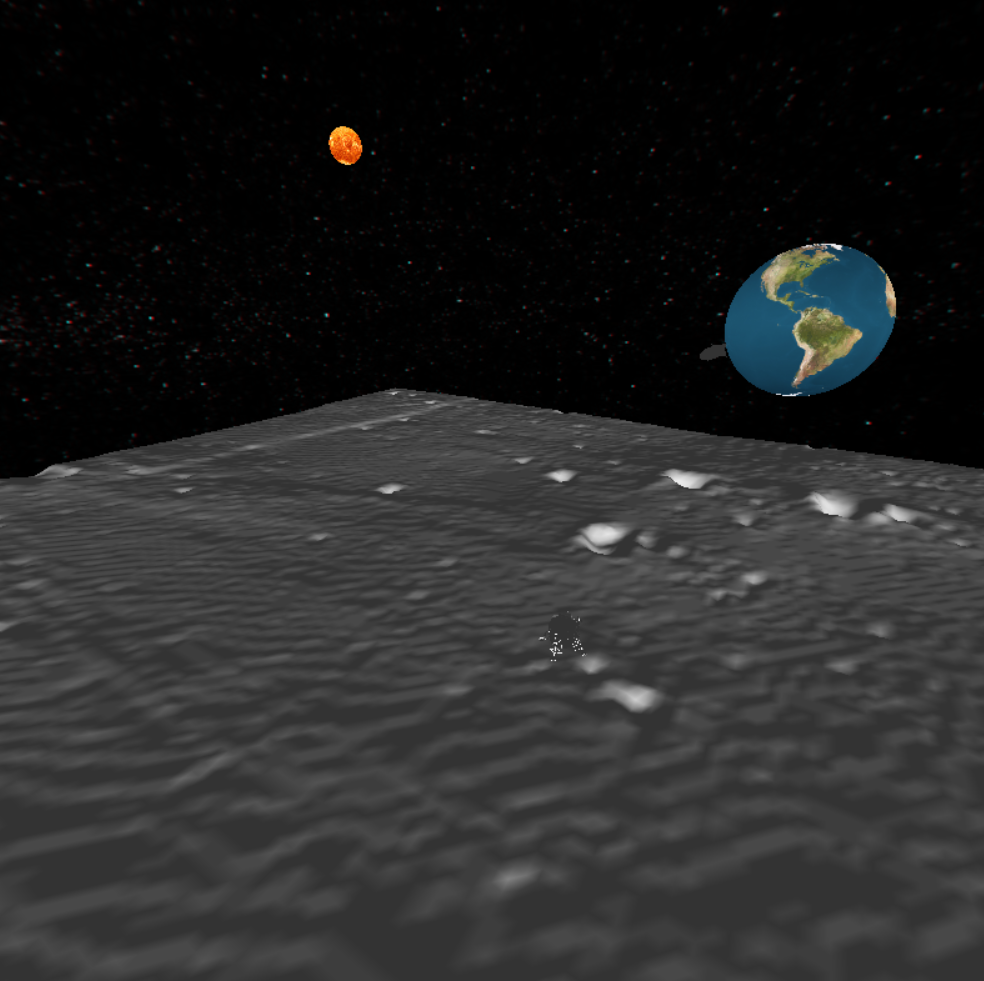
\includegraphics[width=0.5\textwidth]{View1.eps}
    %\caption{Apollo 11 Alpha - View 1: Lunar Surface}
    %\label{fig:View 1}
%\end{wrapfigure}

On Thursday, January 3rd, our design group traveled to OMSI with Mike Bailey to meet with our client, Jim Todd, in person for the first time. We were treated to a full tour of the Harry C. Kendall Planetarium at the Oregon Museum of Science and Industry (OMSI) and got to see the inner workings of their setup, as well as re-defining some of our goals. 

At the time of our visit, our group's plan was to animate all portions of the Apollo 11 mission, from launch to splashdown. However, when talking with Jim, we changed course to instead focus more on what happened on the Moon's surface and instead use original news footage to depict what happened before and after. We have some creative freedom with specifics, but our current story board is now as follows: 

\begin{itemize}
    \item The animation will start with original video of the launch, show a flight path of the Command Module to the Moon, include audio snippets of relevant quotes, and then show the Lunar Lander on the lunar surface.
    
    \item The operator will now be able to interact with the animation, changing the view of the camera on the lunar surface. If no changes are made, the camera will follow a simulation of what Neil Armstrong did on the surface through his eyes. Key points will include: first steps on the surface, planting the American Flag, views of the Earth, and more. During this time, the operator of the planetarium will be able to take questions from the audience. 
    
    \item When the operator is ready to end the animation, they will begin a scripted ending where an astronaut gets back in the Lunar Module and ascends from the surface, show the flight path again, include audio snippets of relevant quotes, and then video of the splashdown on Earth, finishing with credits. 
    
\end{itemize}

Our group will implement this animation in OpenGL for the engineering expo and then translate it to a unique scripting language for use at the planetarium at OMSI. Some functionality, such as including historic video, will not be a feasible accomplishment for the OpenGL program, but will be possible using the Dark Matter planetarium software at OMSI. Any discrepancies between the two versions will be made clear during the engineering expo. 

\section{Current Progress}

As mentioned above, our group traveled to OMSI and received a full tour of the planetarium. We learned that the planetarium received a software upgrade about a year ago and now used DigitalSky: Dark Matter, a software produced by SkySkan, a provider of planetarium equipment and services. Jim showed us the Dark Matter interface on the main control computer and we got to see many different samples. This gave us a much better idea of how our project would look on a domed theater and how to best design the project to make the best use of the theater.

From what we learned from Jim, using the Dark Matter system upgrade will allow us to make full use of the planetarium's capabilities in a more straightforward manor. Mike Bailey has been, and is currently in contact with Jim Todd as well as a contact with SkySkan to find the best ways to complete this conversion. At the end of this term, we will have a sample Dark Matter script ready to test during a trip to the planetarium at OMSI. This will be an indicator to if we are on the right track for getting an animation running in the planetarium. 

As of March 18th, our team has created a program in OpenGL that has the main scene of the Apollo 11 mission on the lunar surface. The lunar surface is placed at the origin and has the lunar module, an astronaut, and an American flag placed on the surface. These objects have been obtained from NASA's 3D object repository online except for the flag, which we modeled. The Moon, Earth, and Sun are included in the scene with a star map making up the background. We were able to accurately position and scaled the Moon and Earth, but the numbers for the Sun had to be manipulated. If we had not changed the numbers, the program would have to use many more resources to accurately represent the true position/scale of the Sun. 


%update later
%audio
%lighting
Currently, there are six viewpoints highlighting different views either on the lunar surface, or from viewpoints in space, each of which are included in this document. These viewpoints are bound to 1-6 on a keyboard. Also, the 'A' key will play an audio clip from the Apollo 11 mission, showing audio functionality.  

\section{To Do}

%To reach the level of alpha, we created the scene in which our animation would be shown. For beta level functionality, we need to make the scene come to life. To do this one of our first goals is to place all objects as accurately as possible, mainly making sure that the landing site is at the correct location on the Moon and that the Earth is at the correct angle when looking from the Moon. Also, currently the Earth is a single texture, but realistically, there are clouds and shadows on the Earth, which will need to be added. There will also be fine tuning to lighting to make the scene on the lunar surface as close to life-like as possible.

%To take this project from a static scene to an animation that can be shown at OMSI, we will focus on adding more viewpoints that are made with key-frame animation so that the viewer is flown throughout the scene. This will be how the operator will mainly show the animation at the expo or OMSI. Then, more audio snippets will be added and our hope it to be able to include historic videos of the Apollo 11 mission. These will give the audience a better idea of what the astronauts and the rest of the world were thinking during this mission. 

%One object that was not included in the alpha was the iconic American flag on the lunar surface. There were no online resources for a 3D object of that flag, so our group will need to make one ourselves. In addition to this, there are other object that we would like to include on the surface such as the various experiment stations that were used; but these are stretch goals because those would be very complex to model without other resources. Then, an overall goal is to make sure that all objects are textured and look as realistic as possible.

\section{Problems and Solutions}

One of the problems our group has encountered obtaining quality 3D objects for our scene. We found that NASA has a GitHub repository that contains .stl files for 3D objects from most of their missions. We obtained the models for the lunar module, astronaut, and lunar surface. However, these models were not to scale, so our group is continuing to adjust their sizes so they are more accurate. Another issue was that textures for the objects were ether incomplete or nonexistent. We are in the process of deciding if we should purchase models of higher quality for Expo. Regardless, Jim Todd will have access to high-quality models and textures for the planetarium. 

Another problem our group has encountered was integrating audio and video into our OpenGl project. For audio, the API we were planning on using uses a heavily deprecated library and the functions to play audio were not working. Instead, our group is currently using a Windows function to play audio files, making it so only computers with Windows OS can play audio. As for video, deprecated libraries were also the culprit, but after talking with Mike Bailey, we decided that our time would be better spent on improving the animation in other areas. For the presentation at OMSI, we are confident that audio and video will not be an issue, so to work towards that end, we are gathering sources for he media. 

Lastly, a more general issue our group encountered was that SkySkan, the company that created the planetarium software, informed us that OpenGL is not directly compatible with their software. We have still decided that creating an OpenGL animation will be a requirement so that we can show something at the engineering expo. While making the animation compatible with the planetarium is still our main focus, for the purposes of priorities, we have moved that to become a stretch goal. That stretch goal is to convert our OpenGL program to a unique scripting language used by the planetarium's software. This should be just like learning a new coding language, but there may also be different functionalities that our team will need to learn and utilize. 

\section{Conclusion}

%Update later
%while some things will be missing from expo, we will make sure they are added to the animation for OMSI
Post launch of our project after the Engineering Expo is when we will focus on the final stages of piping in our animation to OMSI's planetarium, with spring term being dedicated to converting our animation into their in-house scripting language. 

\end{document}